% Harj. Tehtävät luku 3.1
%Ville Tilvis ja Joel Enwald laskivat

\begin{tehtavasivu}

\begin{tehtava}
     Onko lause tosi? 
    \begin{alakohdat}
        \alakohta{$K \subset A$}
        \alakohta{$A \subset V$}
        \alakohta{$V \subset P$}
        \alakohta{$V \subset T$}
    \end{alakohdat}
Merkinnät ovat samat kuin esimerkissä 3.15.
    \begin{vastaus}
    
        \begin{alakohdat}
            \alakohta{On tosi.}
            \alakohta{Ei ole tosi.}
            \alakohta{On tosi.}
            \alakohta{Ei ole tosi.}
        \end{alakohdat}
    \end{vastaus}
\end{tehtava}


\begin{tehtava}
 Olkoot $A = \{7, 8, 9\}$ ja $B=\{5, 6, 7\}$. Määritä joukot
    \begin{alakohdat}
        \alakohta{$A \cup B$,}
        \alakohta{$A \cap B$,}
        \alakohta{$A \setminus B$,}
        \alakohta{$B \setminus A$.}
    \end{alakohdat}

    \begin{vastaus}
    
        \begin{alakohdat}
            \alakohta{$\{5, 6, 7, 8, 9 \}$}
            \alakohta{$\{7\}$}
            \alakohta{$\{8, 9\}$}
            \alakohta{$\{5,6\}$}
        \end{alakohdat}
    \end{vastaus}
\end{tehtava}

\begin{tehtava}
     Olkoot perusjoukko $X$ aakkoset, $A$ vokaalit ja $B=\{x, y, z\}$.
Määritä joukot
    \begin{alakohdat}
        \alakohta{$B\setminus A$,}
        \alakohta{$A\cap B$,}
        \alakohta{$\complement A$,}
        \alakohta{$A \setminus X$.}
    \end{alakohdat}

    \begin{vastaus}
    
        \begin{alakohdat}
            \alakohta{$\{x,z\}$}
            \alakohta{$\{y\}$}
            \alakohta{$\complement A$ on konsonanttien joukko, eli
            $\{b,c,d,f,g,h,j,k,l,m,n,p,q,r,s,t,v,w,x,z \}$}
            \alakohta{$\emptyset$}
        \end{alakohdat}
    \end{vastaus}
\end{tehtava}

\begin{tehtava}
     Olkoot $A$ koulussa opiskelevien täysi-ikäisten opiskelijoiden joukko ja $B$ niiden opiskelijoiden joukko, jotka asuvat vanhempiensa luona. Millaiset opiskelijat kuuluvat joukkoon
    \begin{alakohdat}
        \alakohta{$A \cap B$,}
        \alakohta{$\compl A$,}
        \alakohta{$A \cup \compl B$,}
        \alakohta{$A\setminus B$,}
        \alakohta{$B \setminus A$,}
        \alakohta{$\compl (A \cup B)$?}
    \end{alakohdat}

    \begin{vastaus}
    
        \begin{alakohdat}
    Perusjoukko on koulun opiskelijat.
            \alakohta{Vanhempiensa luona asuvat täysi-ikäiset.}
            \alakohta{Alle täysi-ikäiset.}
            \alakohta{Opiskelijat, jotka ovat täysi-ikäisiä tai eivät asu vanhempiensa luona.}
            \alakohta{Täysi-ikäiset, jotka eivät asu vanhempiensa luona.}
            \alakohta{Vanhempiensa luona asuvat, jotka eivät ole täysi-ikäisiä.}

            \alakohta{Opiskelijat, jotka eivät ole täysi-ikäisiä eivätkä asu vanhempiensa luona.}
        \end{alakohdat}
    \end{vastaus}
    
\end{tehtava}


%\item
%Ilmaise joukkomerkintöjä käyttäen kuvan
%\begin{enumerate}[a)]
%\item keltainen alue,
%\item sininen alue,
%\item violetti alue,
%\item vihreä alue.
%\end{enumerate}
%
%\begin{center}
%
%%% Kuva s. 62
%
%\begin{tikzpicture}[outline/.style={draw=#1,thick}]
%\draw[fill=none] (0,0) rectangle (6.8,4.2);
%\fill[fill=none,outline=black] (2.55,2.1) circle (2);
%\begin{scope}
%\pgfsetfillopacity{0.5}
%\fill[fill=none,outline=black] (4.25,2.1) circle (2);
%\end{scope}
%\draw (.5,3.65) node {\LARGE $X$};
%\draw (2.1,1.0) node {\textcolor{black}{\LARGE $A$}};
%\draw (4.7,1.0) node {\textcolor{black}{\LARGE $B$}};
%\end{tikzpicture}
%
%\end{center}
%%PICXX2

\begin{tehtava}
     Olkoot $A \cap B$, $A \setminus B$ ja $B \setminus A$ epätyhjiä joukkoja. Esitä Venn-diagrammissa varjostettuna alue, joka kuvaa joukkoa
    \begin{alakohdat}
        \alakohta{$\compl (A \cup B)$,}
        \alakohta{$\compl (A \cap B)$,}
        \alakohta{$\compl B \cap A$.}
    \end{alakohdat}

%    \begin{vastaus}
%    FIXME! Näitä kuvia pitää piirtää urakalla. Jotain tällaista:
%\begin{tikzpicture}[outline/.style={draw=#1,thick}]
%\draw[fill=none] (0,0) rectangle (6.8,4.2);
%\fill[fill=none,outline=black] (2.7,2.7) circle (1.4);
%\fill[fill=none,outline=black] (4.1,2.7) circle (1.4);
%\fill[fill=none,outline=black] (3.4,1.5) circle (1.4);
%\draw (.5,3.65) node {\LARGE $X$};
%\draw (1.9,2.9) node {\LARGE $A$};
%\draw (4.9,2.9) node {\LARGE $B$};
%\draw (3.4,.5) node {\LARGE $C$};
%\draw (3.4,3.2) node {$D$};
%\draw (3.4,2.2) node {$E$};
%\draw (3.4,1.1) node {$F$};
%\draw (2.6,1.9) node {$G$};
%\draw (4.2,1.9) node {$G$};
%\end{tikzpicture}
%\def\firstcircle{(0,0) circle (1.5cm)}
%\def\thirdcircle{(0:2cm) circle (1.5cm)}
%
%% Now we can draw the sets:
%\begin{tikzpicture}[outline/.style={draw=#1,thick}]
%    \draw[outline=black] \firstcircle node[below] {\LARGE $A$};
%    \draw[outline=black] \thirdcircle node [below] {\LARGE $B$};
%    \begin{scope}
%      \clip \firstcircle;
%      \fill[green, outline=black] \thirdcircle;
%    \end{scope}
%\end{tikzpicture}
%    \end{vastaus}
    
\end{tehtava}



\begin{tehtava}
     Luokalla on 30 opiskelijaa. Heistä 14 harrastaa jääkiekkoa, 12 jalkapalloa ja 3 molempia. 
    \begin{alakohdat}
        \alakohta{Kuinka moni opiskelija harrastaa pelkkää jääkiekkoa?}
        \alakohta{Kuinka moni opiskelija harrastaa pelkkää jalkapalloa?}
        \alakohta{Kuinka moni opiskelija ei harrasta kumpaakaan?}
    \end{alakohdat}
Vihje: Tilanteesta kannattaa piirtää Venn-diagrammi.
    \begin{vastaus}
    
        \begin{alakohdat}
            \alakohta{11}
            \alakohta{9}
            \alakohta{7}
        \end{alakohdat} %FIXME piirrä Venn-diagrammi
    \end{vastaus}
    
\end{tehtava}


\begin{tehtava}
     Olkoot perusjoukko $\rr$ sekä joukot $A$ ja $B$ reaalilukuvälit $A=[1, 5]$ ja $B=[3, 6]$. Ilmaise välimerkintää käyttäen joukot
    \begin{alakohdat}
        \alakohta{$A \cap B$,}
        \alakohta{$A \cup B$,}
        \alakohta{$A \setminus B$,}
        \alakohta{$\compl A$.}
    \end{alakohdat}

    \begin{vastaus}
    
        \begin{alakohdat}
            \alakohta{$[3,5]$}
            \alakohta{$[1,6]$}
            \alakohta{$[1,3[$}
            \alakohta{$]-\infty,1[ \ \cup \ ]5,\infty[$}
        \end{alakohdat}
    \end{vastaus}
    
\end{tehtava}

\begin{tehtava}
     Yhdistä samaa tarkoittavat lauseet.
\[
\begin{array}{llll}
A & (x\in A)\land (x\in B) & 1 & x\in \complement A \\
B & x\notin A & 2 & x \in A\setminus B \\
C & (x\in A)\lor (x\in B) & 3 & x\in (A\cap B) \\
D & (x\in A)\land (x\notin B) & 4 & x\in (A\cup B)
\end{array}
\]

    \begin{vastaus}
    A3, B1, C4, D2
    \end{vastaus}
    
\end{tehtava}


\begin{tehtava}
     Osoita Venn-diagrammin avulla, että
    \begin{alakohdat}
        \alakohta{\[
A\cup (B \cap C) = (A\cup B)\cap(A\cup C),
\]}
        \alakohta{\[
A\cap (B \cup C) = (A\cap B)\cup(A\cap C).
\]}
    \end{alakohdat}

%    \begin{vastaus}
%    
%        \begin{alakohdat}
%            \alakohta{}
%            \alakohta{}
%        \end{alakohdat}
%    \end{vastaus}
    
\end{tehtava}

\begin{tehtava}
     Sievennä Venn-diagrammin avulla.
    \begin{alakohdat}
        \alakohta{$(B\cap A) \cup (B \cap \compl A)$}
        \alakohta{$\compl (A\cup B) \cup (A \setminus B) \cup (B \setminus A)$}
    \end{alakohdat}

    \begin{vastaus}
    
        \begin{alakohdat}
            \alakohta{$B$}
            \alakohta{perusjoukko}
        \end{alakohdat}
    \end{vastaus}
    
\end{tehtava}

\begin{tehtava}
  Olkoot perusjoukko kokonaislukujen joukko $\zz$, $W$ parillisten kokonaislukujen joukko ja $Y$ luvulla $3$ jaollisten kokonaislukujen joukko. Näitä joukkoja voidaan merkitä $W = \{2n\,|\, n\in\zz\}$ ja $Y = \{3n \,|\, n \in \zz\}$. Määritä joukot   
    \begin{alakohdat}
        \alakohta{$W \cap Y$,}
        \alakohta{$W \setminus Y$,}
        \alakohta{$W \cup Y$.}
    \end{alakohdat}

    \begin{vastaus}
    
        \begin{alakohdat}
            \alakohta{Kuudella jaolliset luvut, eli $\{6n\,|\,n\in\zz\}$}
            \alakohta{Parilliset luvut, jotka eivät ole jaollisia kolmella. $\{2n\,|\,n\in\zz,\,\frac{n}{3}\notin\zz\}$}
            \alakohta{Luvut, jotka ovat jaollisia kahdella tai kolmella. $\{2n,\,3n\,|\,n\in\zz\}$}
        \end{alakohdat}
    \end{vastaus}
    
\end{tehtava}

\begin{tehtava}
     Onko lause tosi?
    \begin{alakohdat}
        \alakohta{$\sqrt{2} \in \rr$}
        \alakohta{$-3 \in \nn$}
        \alakohta{$\pi \in \rr \setminus \qq$}
        \alakohta{$\frac{4}{2} \in \qq \setminus \zz$}
        \alakohta{$\emptyset \subset \zz$}
    \end{alakohdat}

    \begin{vastaus}
    
        \begin{alakohdat}
            \alakohta{On tosi.}
            \alakohta{Ei ole tosi.}
            \alakohta{On tosi.}
            \alakohta{Ei ole tosi.}
            \alakohta{On tosi. Tyhjä joukko on minkä tahansa joukon osajoukko.}
        \end{alakohdat}
    \end{vastaus}
    
\end{tehtava}

\begin{tehtava}
     Määritä joukon
    \begin{alakohdat}
        \alakohta{$\{1, 2\}$}
        \alakohta{$\{1, 2, 3\}$}
    \end{alakohdat}
kaikki osajoukot.
    \begin{vastaus}
    
        \begin{alakohdat}
            \alakohta{$\emptyset$, $\{1\}$, $\{2\}$, $\{1, 2\}$}
            \alakohta{$\emptyset$, $\{1\}$, $\{2\}$, $\{3\}$,
             $\{1, 2\}$, $\{1, 3\}$, $\{2, 3\}$, $\{1, 2, 3\}$}

        \end{alakohdat}
    \end{vastaus}
    
\end{tehtava}

\begin{tehtava}
*
Joukon $A$ \termi{potenssijoukko}{potenssijoukoksi} $\mathcal{P}(A)$ kutsutaan kaikkien joukon $A$ osajoukkojen muodostamaa joukkoa:
\[
\mathcal{P}(A)=\{ B \, | \, B\subset A\}.
\]
    \begin{alakohdat}
        \alakohta{Määritä joukon $\{1, 2, 3\}$ potenssijoukko.}
        \alakohta{Määritä tyhjän joukon $\emptyset$ potenssijoukko.}
        \alakohta{Joukko $\{\emptyset\}$ on joukko, jonka ainut alkio on tyhjä joukko.Määritä joukon $\{\emptyset\}$ potenssijoukko.}
    \end{alakohdat}

    \begin{vastaus}
    
        \begin{alakohdat}
            \alakohta{$\{ \emptyset, \{1\}, \{2\}, \{3\},
             \{1, 2\}, \{1, 3\}, \{2, 3\}, \{1, 2, 3\}\}$}
            \alakohta{$\{ \emptyset\}$}
            \alakohta{$\{\emptyset, \{\emptyset\} \}$}
        \end{alakohdat}
    \end{vastaus}
    
\end{tehtava}

\begin{tehtava}
    *
Luonnolliset luvut voidaan tulkita joukko-opillisesti käyttämällä edellisessä tehtävässä esitettyä potenssijoukon käsitettä. Ajatuksena on, että lukua $0$ vastaa tyhjä joukko $\emptyset$ ja kutakin luonnollista lukua $n + 1$ vastaava joukko on luonnollista lukua $n$ vastaavan joukon potenssijoukko. Siis esimerkiksi lukua $1$ vastaa tyhjän joukon $\emptyset$ potenssijoukko $\mathcal{P}(\emptyset)$, lukua $2$ potenssijoukko $\mathcal{P}(\mathcal{P}(\emptyset))$ ja niin edelleen. 
    \begin{alakohdat}
        \alakohta{Määritä lukuja $3$ ja $4$ vastaavat joukot.}
        \alakohta{Mitä luonnollista lukua vastaa joukko $\{\emptyset,\{\emptyset\}\}$?}
        \alakohta{Vastaako joukko $\{\{\emptyset\}\}$ jotakin luonnollista lukua?}
    \end{alakohdat}

    \begin{vastaus}
    
        \begin{alakohdat}
            \alakohta{Lukua yksi vastaa joukko $\{\emptyset\}$,
			lukua kaksi $\{\emptyset, \{\emptyset\} \}$, lukua kolme            
             $\{ \ \emptyset, \{\emptyset\}, \{ \{ \emptyset \}\}, 
             \{ \emptyset, \{\emptyset \} \} \ \}$ ja lukua neljä \\
            $\{ \ \ \emptyset, % 0 alkiota
            \{\emptyset \},
            \{ \{\emptyset \} \}, \{\{\{\emptyset \}\}\}, \{\{ \emptyset, \{\emptyset \} \} \},$  \\ % 1 alkio valmis
			\ $ \{\emptyset, \{\emptyset\} \},
            \{\emptyset,  \{ \{ \emptyset \}\} \},
			\{\emptyset,  \{ \emptyset, \{\emptyset \} \} \},$ \\ 
			\ $ \{\{\emptyset\},  \{ \{ \emptyset \}\}\},  
			\{\{\emptyset\}, \{ \emptyset, \{\emptyset \} \} \},
			\{ \{ \{ \emptyset \}\}, 
              \{ \emptyset, \{\emptyset \} \} \},$ \\ % 2 alkiota valmis
			 \ $ \{ \ \emptyset, \{\emptyset\}, \{ \{ \emptyset \}\}\},$ \\
			 \ $ \{ \emptyset, \{\emptyset\}, 
             \{ \emptyset, \{\emptyset \} \} \}, $  \\ 	
             \ $ \{ \emptyset, \{ \{ \emptyset \}\}, 
             \{ \emptyset, \{\emptyset \} \} \}, $  \\
             \ $ \{\{\emptyset\}, \{ \{ \emptyset \}\}, 
             \{ \emptyset, \{\emptyset \} \} \},$  \\  %3 alkiota valmis 
             \ $  \{  \emptyset, \{\emptyset\}, \{ \{ \emptyset \}\}, 
             \{ \emptyset, \{\emptyset \} \} \} \ \ \}$.}
             \alakohta{Lukua kaksi.}
            \alakohta{Ei vastaa.}
        \end{alakohdat}
    \end{vastaus}
    
\end{tehtava}

\end{tehtavasivu}
\begin{kotitehtavasivu}

\begin{tehtava}
Olkoot $A = \{a, b, c, d\}$ ja $B=\{a, c, e\}$. Määritä joukot
    \begin{alakohdat}
        \alakohta{$A \cup B$,}
        \alakohta{$A \cap B$,}
        \alakohta{$A \setminus B$,}
        \alakohta{$B \setminus A$.}                
    \end{alakohdat}

    \begin{vastaus}
    
        \begin{alakohdat}
        \alakohta{$\{a, b, c, d, e\}$}
        \alakohta{$\{a, c\}$}
        \alakohta{$\{a, b, d\}$}
        \alakohta{$\{e\}$} 
        \end{alakohdat}
    \end{vastaus}
\end{tehtava}

\begin{tehtava}
Onko lukujoukkoja koskeva lause tosi?
    \begin{alakohdat}
        \alakohta{$\zz \subset \nn$}
        \alakohta{$\zz \subset \qq$}
        \alakohta{$\rr \subset \zz$}
        \alakohta{$\qq \subset \nn$}
        \alakohta{$\qq \subset \qq$}             
    \end{alakohdat}

    \begin{vastaus}
    
        \begin{alakohdat}
        \alakohta{Ei ole tosi.}
        \alakohta{On tosi.}
        \alakohta{Ei ole tosi.}
        \alakohta{Ei ole tosi.}
        \alakohta{On tosi.} 
        \end{alakohdat}
    \end{vastaus}
\end{tehtava}


\begin{tehtava}
Olkoot perusjoukko $X$ aakkoset, $A=\{j, o, k, u\}$, $B=\{k, o, j, u\}$ ja $C=\{k, a, j, o\}$. Määritä joukot
    \begin{alakohdat}
        \alakohta{$A\setminus B$,}
        \alakohta{$(A\cap B)\cup C$,}
        \alakohta{$A\setminus \complement (B\cup C)$.}
     \end{alakohdat}

    \begin{vastaus}
    
        \begin{alakohdat}
        \alakohta{$\emptyset$}
        \alakohta{$\{j, o, k, u, a, o\}$}
        \alakohta{$\{j, o, k, u\}$}
        \end{alakohdat}
    \end{vastaus}
\end{tehtava}


\begin{tehtava}
 Olkoot $X$ perusjoukko ja $A$ jokin perusjoukon osajoukko. Sievennä.
    \begin{alakohdat}
        \alakohta{$A\cup \emptyset$}
        \alakohta{$A\cap \emptyset$}
        \alakohta{$A\cap X$}
        \alakohta{$A\cup X$}                
    \end{alakohdat}

    \begin{vastaus}
    
        \begin{alakohdat}
        \alakohta{$A$}
        \alakohta{$\emptyset$}
        \alakohta{$A$}
        \alakohta{$X$} 
        \end{alakohdat}
    \end{vastaus}
\end{tehtava}


\begin{tehtava}
Olkoot $A \subset B$ ja $B \setminus A$ epätyhjä. Esitä Venn-diagrammissa varjostettuna alue, joka kuvaa joukkoa
    \begin{alakohdat}
        \alakohta{$B \setminus A$,}
        \alakohta{$\compl A \cap B$,}
        \alakohta{$A \cup \compl B$.}                
    \end{alakohdat}

%    \begin{vastaus} %FIXME: Venn-diagrammi
%    
%        \begin{alakohdat}
%        \alakohta{}
%        \alakohta{}
%        \alakohta{} 
%        \end{alakohdat}
%    \end{vastaus}
\end{tehtava}


\begin{tehtava}
Olkoon perusjoukko $X$ kaikkien kalenterivuoden päivien joukko. Olkoot $A$ arkipäivien (maanantai--perjantai) joukko, $L$ liputuspäivien joukko ja $T$ toukokuulle ajoittuvien päivien joukko. Millaiset päivät kuuluvat joukkoon
    \begin{alakohdat}
        \alakohta{$\compl A$}
        \alakohta{$L \cap \compl T$}
        \alakohta{$L \setminus A$}
        \alakohta{$T \setminus (A \cup L)$} 
        \alakohta{$\compl (A \cup L \cup T)$?}               
    \end{alakohdat}

    \begin{vastaus}
    
        \begin{alakohdat}
        \alakohta{Lauantait ja sunnuntait.}
        \alakohta{Muut kuin toukokuun liputuspäivät.}
        \alakohta{Lauantaiden ja sunnuntaiden liputuspäivät.}
        \alakohta{Toukokuun lauantait ja sunnuntait, jotka
        eivät ole liputuspäiviä.} 
        \alakohta{Lauantait ja sunnuntait, jotka eivät ole
        liputuspäiviä eivätkä ole toukokuussa.} 
        \end{alakohdat}
    \end{vastaus}
\end{tehtava}

\begin{tehtava}
Onko lause tosi?
    \begin{alakohdat}
        \alakohta{$0 \in \{0, 1, 2\}$}
        \alakohta{$\{0\} \subset \{0, 1, 2\}$}
        \alakohta{$\emptyset \subset \{1, 2\}$}
        \alakohta{$\{\textrm{å}, \textrm{ä}, \textrm{ö}\} \subset \{\textrm{o}, \textrm{ä}, \textrm{ö}\}$}                
    \end{alakohdat}

    \begin{vastaus}
    
        \begin{alakohdat}
        \alakohta{On.}
        \alakohta{On.}
        \alakohta{On.}
        \alakohta{Ei.} 
        \end{alakohdat}
    \end{vastaus}
\end{tehtava}


\begin{tehtava}
Luokan opiskelijoista kahdeksalla on läppäri, kymmenellä pöytäkone ja
viidellä tabletti.
Kahdella opiskelijalla on sekä läppäri että pöytäkone, kolmella sekä
tabletti että pöytäkone, mutta kellään ei ole sekä läppäriä että
tablettia. Kahdella opiskelijalla ei ole mitään tietokonetta.
    \begin{alakohdat}
        \alakohta{Piirrä tilannetta kuvaava Venn-diagrammi.}
        \alakohta{Kuinka monella opiskelijalla on läppäri mutta ei pöytäkonetta?}
        \alakohta{Kuinka monella opiskelijalla on vain pöytäkone?}
        \alakohta{Kuinka monta opiskelijaa luokalla on?}                
    \end{alakohdat}

    \begin{vastaus}
    
        \begin{alakohdat}
        \alakohta{-} % FIXME : lisää kuva
        \alakohta{6}
        \alakohta{5}
        \alakohta{20} 
        \end{alakohdat}
    \end{vastaus}
\end{tehtava}

\begin{tehtava}
Olkoot perusjoukko $\rr$ sekä joukot $A$ ja $B$ reaalilukuvälit $A=]-1, 2[$ ja $B=[0, 4[$. Ilmaise välimerkintää käyttäen joukot
    \begin{alakohdat}
        \alakohta{$A \cup B$,}
        \alakohta{$A \cap B$,}
        \alakohta{$\compl (A \cap B)$,}
        \alakohta{$B \setminus A$,}
        \alakohta{$B \setminus (A \cap B)$,}
        \alakohta{$A \cap \compl B$.}                        
    \end{alakohdat}

    \begin{vastaus}
    
        \begin{alakohdat}
        \alakohta{}
        \alakohta{}
        \alakohta{}
        \alakohta{}
        \alakohta{}
        \alakohta{} 
        \end{alakohdat}
    \end{vastaus}
\end{tehtava}


\begin{tehtava}
Osoita Venn-diagrammin avulla, että
    \begin{alakohdat}
        \alakohta{\[
X\setminus (A\cup B) = (X\setminus A)\cap (X\setminus B),
\]}
        \alakohta{\[
X \setminus (A\cap B) = (X\setminus A)\cup (X\setminus B).
\]}
      
    \end{alakohdat}

    \begin{vastaus}
    
        \begin{alakohdat}
        \alakohta{}
        \alakohta{}
        \end{alakohdat}
    \end{vastaus}
\end{tehtava}


\begin{tehtava}
Jos $A\subset B$ ja $B\subset C$, niin mitä voidaan päätellä joukoista $A$ ja $C$? Perustele 
    \begin{alakohdat}
        \alakohta{Venn-diagrammin avulla,}
        \alakohta{osajoukon määritelmän avulla.}
    \end{alakohdat}

    \begin{vastaus}
    
        \begin{alakohdat}
        \alakohta{}
        \alakohta{}
        \end{alakohdat}
    \end{vastaus}
\end{tehtava}


\begin{tehtava}
Onko lause tosi?
    \begin{alakohdat}
        \alakohta{$A \cap B \subset A$}
        \alakohta{$\compl (\compl A) = A$}
        \alakohta{$(A\cup B) \setminus B = A$}
        \alakohta{$A \cap \compl B = A \setminus B$}   
        \alakohta{$$B \cap \compl B = B$$}             
    \end{alakohdat}

    \begin{vastaus}
    
        \begin{alakohdat}
        \alakohta{}
        \alakohta{}
        \alakohta{}
        \alakohta{} 
        \alakohta{}
        \end{alakohdat}
    \end{vastaus}
\end{tehtava}


\begin{tehtava}
Tarkastellaan kaksinumeroisia luonnollisia lukuja $10, 11, \ldots, 98, 99$.
    \begin{alakohdat}
        \alakohta{Kuinka monta kaksinumeroista luonnollista lukua on olemassa?}
        \alakohta{Kuinka moni niistä on jaollinen luvulla $4$? Kuinka moni ei ole jaollinen luvulla $4$?}
        \alakohta{Kuinka moni kaksinumeroisista luonnollisista luvuista on jaollinen luvulla $6$?}
        \alakohta{Kuinka moni kaksinumeroisista luonnollisista luvuista on jaollinen luvuilla $4$ ja $6$?}    
        \alakohta{Kuinka moni kaksinumeroisista luonnollisista luvuista on jaollinen luvulla $4$ tai luvulla $6$?}
        \alakohta{Kuinka moni kaksinumeroisista luonnollisista luvuista ei ole jaollinen luvulla $4$ eikä luvulla $6$?}  
        \alakohta{Piirrä tilanteesta Venn-diagrammi.}          
    \end{alakohdat}

    \begin{vastaus}
    
        \begin{alakohdat}
        \alakohta{}
        \alakohta{}
        \alakohta{}
        \alakohta{} 
        \alakohta{}
        \alakohta{}
        \alakohta{}         
        \end{alakohdat}
    \end{vastaus}
\end{tehtava}



\begin{tehtava}
Merkitään kuvan ympyröiden sisään jääviä joukkoja kirjaimilla $A$, $B$ ja $C$. Ilmaise joukkomerkintöjä käyttäen joukkojen $A$, $B$ ja $C$ avulla kuvan
    \begin{alakohdat}
        \alakohta{alue $D$,}
        \alakohta{alue $E$,}
        \alakohta{alue $F$,}
        \alakohta{alue $G$.}                
    \end{alakohdat}
\medskip

\begin{center}
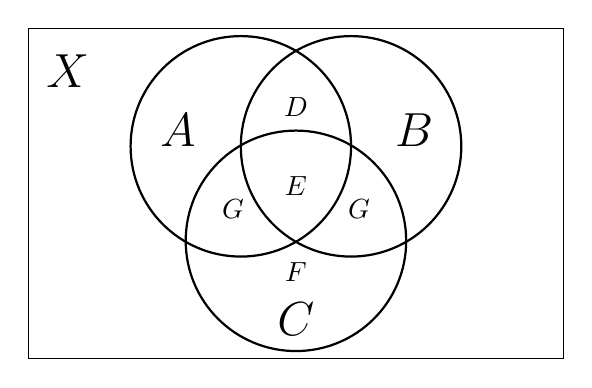
\begin{tikzpicture}[outline/.style={draw=#1,thick}]
\draw[fill=none] (0,0) rectangle (6.8,4.2);
\fill[fill=none,outline=black] (2.7,2.7) circle (1.4);
\fill[fill=none,outline=black] (4.1,2.7) circle (1.4);
\fill[fill=none,outline=black] (3.4,1.5) circle (1.4);
\draw (.5,3.65) node {\LARGE $X$};
\draw (1.9,2.9) node {\LARGE $A$};
\draw (4.9,2.9) node {\LARGE $B$};
\draw (3.4,.5) node {\LARGE $C$};
\draw (3.4,3.2) node {$D$};
\draw (3.4,2.2) node {$E$};
\draw (3.4,1.1) node {$F$};
\draw (2.6,1.9) node {$G$};
\draw (4.2,1.9) node {$G$};
\end{tikzpicture}
\end{center}

\medskip
    \begin{vastaus}
    
        \begin{alakohdat}
        \alakohta{}
        \alakohta{}
        \alakohta{}
        \alakohta{} 
        \end{alakohdat}
    \end{vastaus}
\end{tehtava}

\end{kotitehtavasivu}
